\documentclass[pscyr]{hedlab}
\usepackage[russian]{babel}
\usepackage{graphicx}
\graphicspath{{images/}}
\usepackage{listings}

\lstset{
    basicstyle=\footnotesize,
    inputencoding=utf8,
    extendedchars=True,
    language=[Sharp]C,
    numbers=left,
    numberstyle=\footnotesize,
    breakatwhitespace=\false,
    breaklines=True,
    tabsize=2,
    keepspaces=true,
}

\labname{Аутентификация и авторизация в Web-приложениях}
\labnum{6}
\student{Голубев~А.~В., САПР-1.1п}
\labdate{}

\begin{document}
    \makeheader
    \emph{Цель:} получение практических навыков создания безопасных ASP.NET приложений с 
    использованием механизмов аутентификации и авторизации.\\
    \emph{Задачи:} 
    \begin{itemize}
        \item Создать ASP.NET приложение, осуществляющее аутентификацию пользователя, и настроить 
            web.config файл в соответствии с заданием.
    \end{itemize}
    Для создания аутентификации был использована библиотека Owin.\\
    Код регистрации:
    \lstinputlisting{./code/register.cs}
    \pagebreak
    Код авторизации:
    \lstinputlisting{./code/login.cs}
    \pagebreak
    Конфигурация:
    \lstinputlisting{./code/startup.cs}
    \pagebreak
    Страница авториазции:
    \lstinputlisting[inputencoding=utf8,basicstyle=\footnotesize,language=HTML]{./code/login.aspx}

    \pagebreak

    Скриншоты Web-страниц:
    \begin{figure}[h!]
        \center
        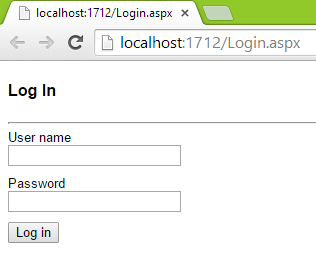
\includegraphics[width=.47\textwidth]{lab06_01} \hspace{1em}
        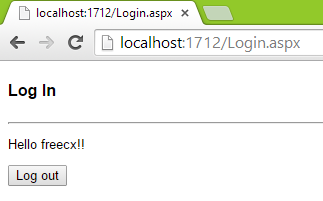
\includegraphics[width=.47\textwidth]{lab06_02} \\
        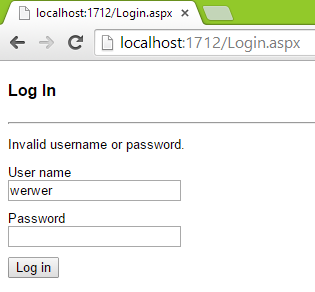
\includegraphics[width=.47\textwidth]{lab06_03} \hspace{1em}
        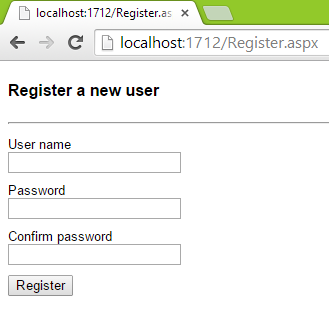
\includegraphics[width=.47\textwidth]{lab06_04}
    \end{figure}

    \emph{Вывод:} в результате проделанной работы
    \begin{itemize}
        \item Создал ASP.NET приложение, осуществляющее аутентификацию пользователя, и настроили 
            web.config файл в соответствии с заданием.
    \end{itemize}
\end{document}